\chapter{Realizacja założeń projektowych}\label{cha:rzp}

%---------------------------------------------------------------------------

\section{Wprowadzenie}\label{sec:wprowadzenie}


Promowany w~latach 80-tych ruch wolnego oprogramowania~\cite{b23} znacząco wpłynął na rozwój aplikacji i~algorytmów. Powszechny dostęp do Internetu umożliwił upublicznianie kodów źródłowych, co zrzeszało duże społeczności pracujące wspólnie nad rozwojem programów komputerowych. Otwarte bazy aplikacji i~algorytmów pozwoliły niezależnym programistom  na wykorzystanie ich do rozwoju kolejnych w~wydajniejszy sposób. Realizacja projektu niniejszej pracy stanowi bazę, która może zostać wykorzystana w~podobny sposób. Kod tej aplikacji może zostać łatwo zaadaptowany do połączenia jej z innym oprogramowaniem. Możliwe też jest wprowadzenie modyfikacji algorytmu metody źródeł pozornych  lub zaimplementowanie dodatkowych metod wewnątrz aplikacji.


Aplikacja została napisana przy użyciu OpenCL w~wersji 1.2. Zdecydowano się na starszą wersję ze względu na kompatybilność z wieloma popularnymi urządzeniami. Platforma została napisana przy użyciu języka C++11. Zarówno dane wejściowe jak i~wyjściowe transferowane są między plikiem wykonywalnym a~plikami tekstowymi. Dane przechowywane są w zmiennych o pojedynczej precyzji. Zmniejsza to czas obliczeń na urządzeniach o architekturze 32-bitowej i wprowadza wystarczająco mały błąd dla tego typu obliczeń.



%---------------------------------------------------------------------------

\section{Implementacja algorytmu}\label{sec:ra}

Aplikacja do obliczeń używa jednej platformy (Kod~źr.~2.), która definiuje jeden kontekst obliczeniowy i~jedno urządzenie.

\begin{program}[H]
\caption{Definiowanie platformy}
\begin{lstlisting}
cl_platform_id* platforms = new cl_platform_id[numPlatforms];
status = clGetPlatformIDs(numPlatforms, platforms, NULL);
\end{lstlisting}
\end{program}

Dane wejściowe alokowane są w~pamięci po stronie platformy. Następnie tworzony jest kontekst obliczeniowy (Kod~źr.~3.), który przy użyciu predyrektywy \verb|CL_PRESENT_DEVICE| wybiera , jaki typ urządzenia zostanie wybrany.

\begin{program}[H]
\caption{Definiowanie kontekstu obliczeniowego}
\begin{lstlisting}
cl_context_properties cps[3] = { CL_CONTEXT_PLATFORM, (cl_context_properties)platform, 0 };
context = clCreateContextFromType(
                                  cps, 
                                  CL_PRESENT_DEVICE, 
                                  NULL, 
                                  NULL, 
                                  &status);
\end{lstlisting}
\end{program}

Następuje poszukiwanie urządzenia o zadanym typie i~zapisanie informacji o nim (Kod~źr.~4.).

\begin{program}[H]
\caption{Pobieranie listy dostępnych urządzeń}
\begin{lstlisting}
clGetContextInfo(
                 context, 
                 CL_CONTEXT_DEVICES, 
                 deviceListSize, 
                 devices, 
                 NULL);

\end{lstlisting}
\end{program}

Kolejnym krokiem jest przygotowanie kolejki zadań (Kod~źr.~5.). Posłuży ona do stworzenia przestrzeni indeksowania dla wątków.

\begin{program}[H]
\caption{Przygotowanie kolejki zadań}
\begin{lstlisting}
commandQueue = clCreateCommandQueue(
                                    context, 
                                    devices[0], 
                                    0, 
                                    &status);
\end{lstlisting}
\end{program}

Dane wejściowe przekazywane są do kontekstu obliczeniowego poprzez bufory (Kod~źr.~6.). Oddzielne bufory dla każdej danej wejściowej transferują owe  dane do zdefiniowanego przez kernel miejsca w~pamięci. 

\begin{program}[H]
\caption{Definicja buforu danych dla parametru plA}
\begin{lstlisting}

plABuffer = clCreateBuffer(
                           context, 
                           CL_MEM_READ_WRITE | CL_MEM_USE_HOST_PTR,
                           sizeof(cl_float) * walls,
                           plA, 
                           &status);
\end{lstlisting}
\end{program}

Kod kernela przechowywany jest w~postaci oddzielnego pliku tekstowego~(załącznik~A). Jest on kompilowany przez bibliotekę OpenCL podczas wykonywania głównego programu. Plik ten jest wczytywany przez platformę, a~następnie budowany do obiektu (Kod~źr.~7.), który później będzie wywoływany przez poszczególne wątki. Kod kernela zawiera implementację algorytmu metody źródeł pozornych (Rysunek 5.1.), który na podstawie danych z kontekstu obliczeniowego wykonuje obliczenia dla jednej wariacji powierzchni odbijających. Ilość wszystkich wariacji powierzchni odbijających dla $N$ powierzchni i~$L$ rzędu źródeł pozornych wynosi $N^L$. Przestrzeń indeksowania stanowi kolejne liczby od 1 do $N^L$. Dla każdego wątku indeks przedstawiany jest w~postaci liczby w~systemie liczbowym o podstawie N. Każda kolejna cyfra takiej liczby odpowiada poszczególnej płaszczyźnie, dzięki czemu dla każdego indeksu uzyskujemy unikatową wariację powierzchni odbijających (Rysunek 5.2.).

\begin{figure}[H]
        \centering
                \centering
                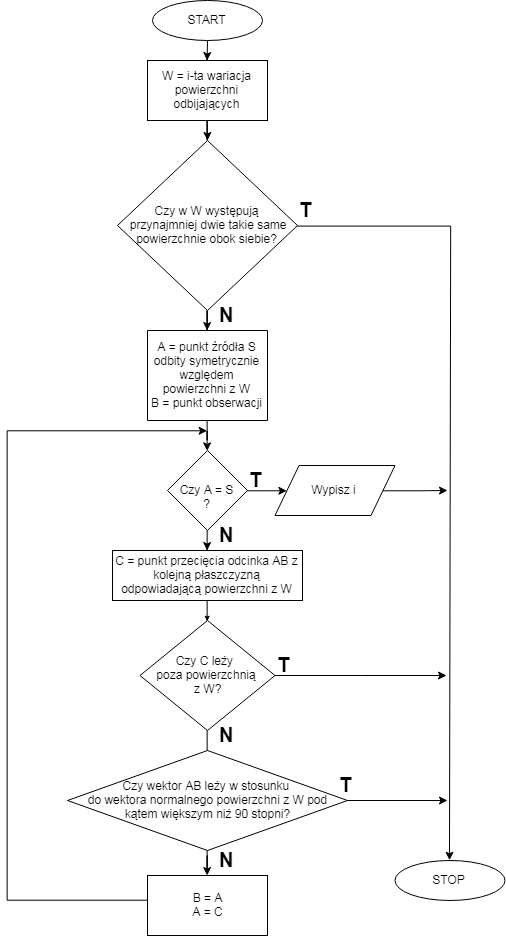
\includegraphics[width=12cm]{kerneldiagram}
	\caption{Schemat blokowy algorytmu metody źródeł pozornych dla pojedyńczej wariacji powierzchni odbijających.}
\end{figure}

\begin{figure}[H]
        \centering
                \centering
                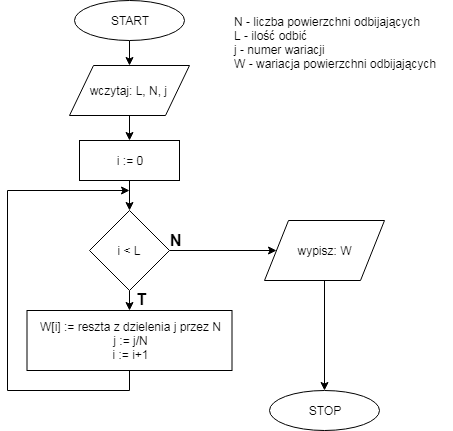
\includegraphics[width=12cm]{wariacja}
	\caption{Schemat blokowy wyznaczania j-tej wariacji powierzchni odbijających.}
\end{figure}

\begin{program}[H]
\caption{Budowanie obiektu kernela}
\begin{lstlisting}
program = clCreateProgramWithSource(
                                    context, 
                                    1, 
                                    &source,
                                    sourceSize,
                                    &status);
status = clBuildProgram(program, 1, devices, NULL, NULL, NULL);
kernel = clCreateKernel(program, "templateKernel", &status);
\end{lstlisting}
\end{program}

W zależności od wykorzystywanego urządzenia należy dobrać odpowiednio wielkości grup wątków. Zostały one zdefiniowane w~zmiennych globalThreads i~localThreads. Należy zwrócić uwagę, aby nie przekraczały one maksymalnych dopuszczalnych wartości dla danego urządzenia. W tym celu pobierane są informacje z bieżącego urządzenia o maksymalnych dopuszczalnych wartościach (Kod~źr.~8.).

\begin{program}[H]
\caption{Pobranie informacji o zasobach urządzenia}
\begin{lstlisting}
clGetDeviceInfo(
                devices[0], 
                CL_DEVICE_MAX_WORK_GROUP_SIZE, 
                sizeof(size_t), 
                (void*)&maxWorkGroupSize, 
                NULL);
clGetDeviceInfo(
                devices[0], 
                CL_DEVICE_MAX_WORK_ITEM_DIMENSIONS, 
                sizeof(cl_uint), 
                (void*)&maxDims, 
                NULL);
clGetDeviceInfo(
                devices[0], 
                CL_DEVICE_MAX_WORK_ITEM_SIZES, 
                sizeof(size_t)*maxDims,
                (void*)maxWorkItemSizes,
                NULL);
\end{lstlisting}
\end{program}

Przed uruchomieniem kernela przekazywany jest do niego bufor danych (Kod~źr.~9.).

\begin{program}[H]
\caption{Przekazanie bufora plABuffer do kernela}
\begin{lstlisting}

clSetKernelArg(
               kernel, 
               1, 
               sizeof(cl_mem), 
               (void *)&plABuffer);
\end{lstlisting}
\end{program}

Następuje uruchomienie kolejki zadań i~czekanie na ich wykonanie (Kod~źr.~10.). Po wykonaniu zadań kolejka zostaje zwolniona.

\begin{program}[H]
\caption{Uruchomienie kolejki zadań dla bufora wejściowego}
\begin{lstlisting}
clEnqueueNDRangeKernel(
                       commandQueue,
                       kernel,
                       1,
                       NULL,
                       globalThreads,
                       localThreads,
                       0,
                       NULL,
                       &events[0]);
clWaitForEvents(1, &events[0]);
clReleaseEvent(events[0]);
\end{lstlisting}
\end{program}

Następnie dane wyjściowe odczytywane są z bufora wyjściowego (Kod~źr.~11.)

\begin{program}[H]
\caption{Uruchomienie kolejki zadań dla bufora wyjściowego}
\begin{lstlisting}
clEnqueueReadBuffer(
                    commandQueue,
                    outputBuffer,
                    CL_TRUE,
                    0,
                    width * sizeof(cl_uint),
                    output,
                    0,
                    NULL,
                    &events[1]);
\end{lstlisting}
\end{program}


%---------------------------------------------------------------------------

\section{Obsługa aplikacji}\label{sec:oa}

Przed kompilacją programu należy przygotować kod pod urządzenia, na jakich  będzie on wykonywany. W zależności od typu procesora należy zdefiniować dyrektywę \verb|CL_PRESENT_DEVICE| jako \verb|CL_DEVICE_TYPE_CPU| dla procesorów, lub \verb|CL_DEVICE_TYPE_GPU| dla kart graficznych. W zależności od parametrów urządzenia należy odpowiednio zdefiniować rozmiary grup wątków w~zmiennych localThreads i~globalThreads, a~następne skompilować do pliku wykonywalnego dołączając biblioteki standardu OpenCL. Plik wykonywalny przyjmuje dane w~postaci pliku wejściowego o nazwie input.txt. W danym pliku należy zdefiniować w~kolejnych liniach  rząd pozornych źródeł, współrzędne punktu źródła dźwięku i~punktu obserwacji, współczynniki płaszczyzn powierzchni odbijających w~postaci ogólnej, granice powierzchni dla poszczególnych osi oraz współczynniki pochłaniania dźwięku dla każdej powierzchni (Kod~źr.~12).

\begin{program}[H]
\caption{Plik wejściowy programu}
\begin{lstlisting}
3              %rząd siatki źródeł pozornych
0.2, 0.4, 0.3  % współrzędne punktu źródła
0.6, -1.7, 0.4 % współrzędne punktu obserwacji
0, 0, 1, 3.3   % współczynniki płaszczyzny dla pierwszej powierzchni odbijającej 
-2, -7, -3.3   % dolne granice powierzchni dla osi x, y i~z 
2, 7, -3.3     % gorne granice powierzchni dla osi x, y i~z
0.71           % współczynnik pochłaniania powierzchni
\end{lstlisting}
\end{program}

Dane wyjściowe otrzymywane są w~postaci pliku output.txt. Po wykonaniu obliczeń w~pliku znajdują się współrzędne punktów siatki źródeł pozornych wraz z ich energią.

Przy ustawieniu dyrektywy \verb|write_file| na $true$ i~wybraniu kombinacji powierzchni odbijających program wygeneruje plik ze skryptem wejściowym do programu GeoGebra. Wygenerowany skrypt rysuje trójwymiarową grafikę (Rys. 5.3.), na której znajdują się powierzchnie odbijające, punkt źródła dźwięku, punkt pozornego źródła, punkt obserwacji oraz ścieżka promienia dźwiękowego.

\begin{figure}[H]
        \centering
                \centering
                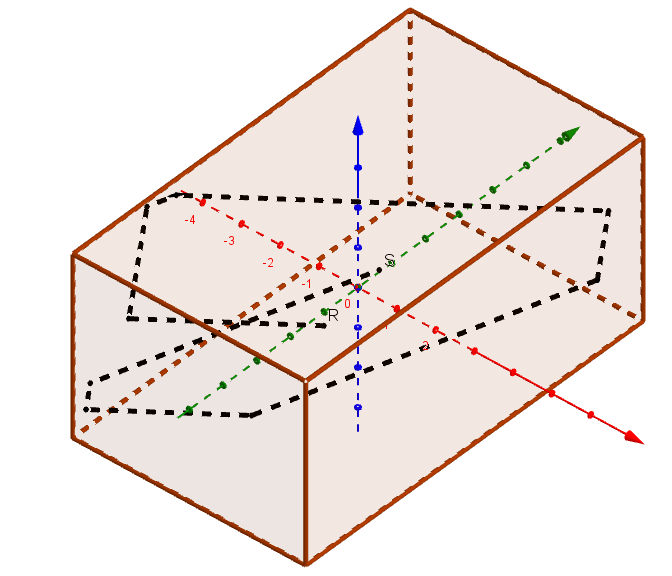
\includegraphics[width=12cm]{rys10}
	\caption{Ścieżka promienia dźwiękowego (S - punkt źródła dźwięku, R - punkt obserwacji).}
\end{figure}

Dane z pliku output.txt mogą posłużyć do wygenerowania siatki źródeł pozornych (Rys. 5.4.).

\begin{figure}[H]
        \centering
                \centering
                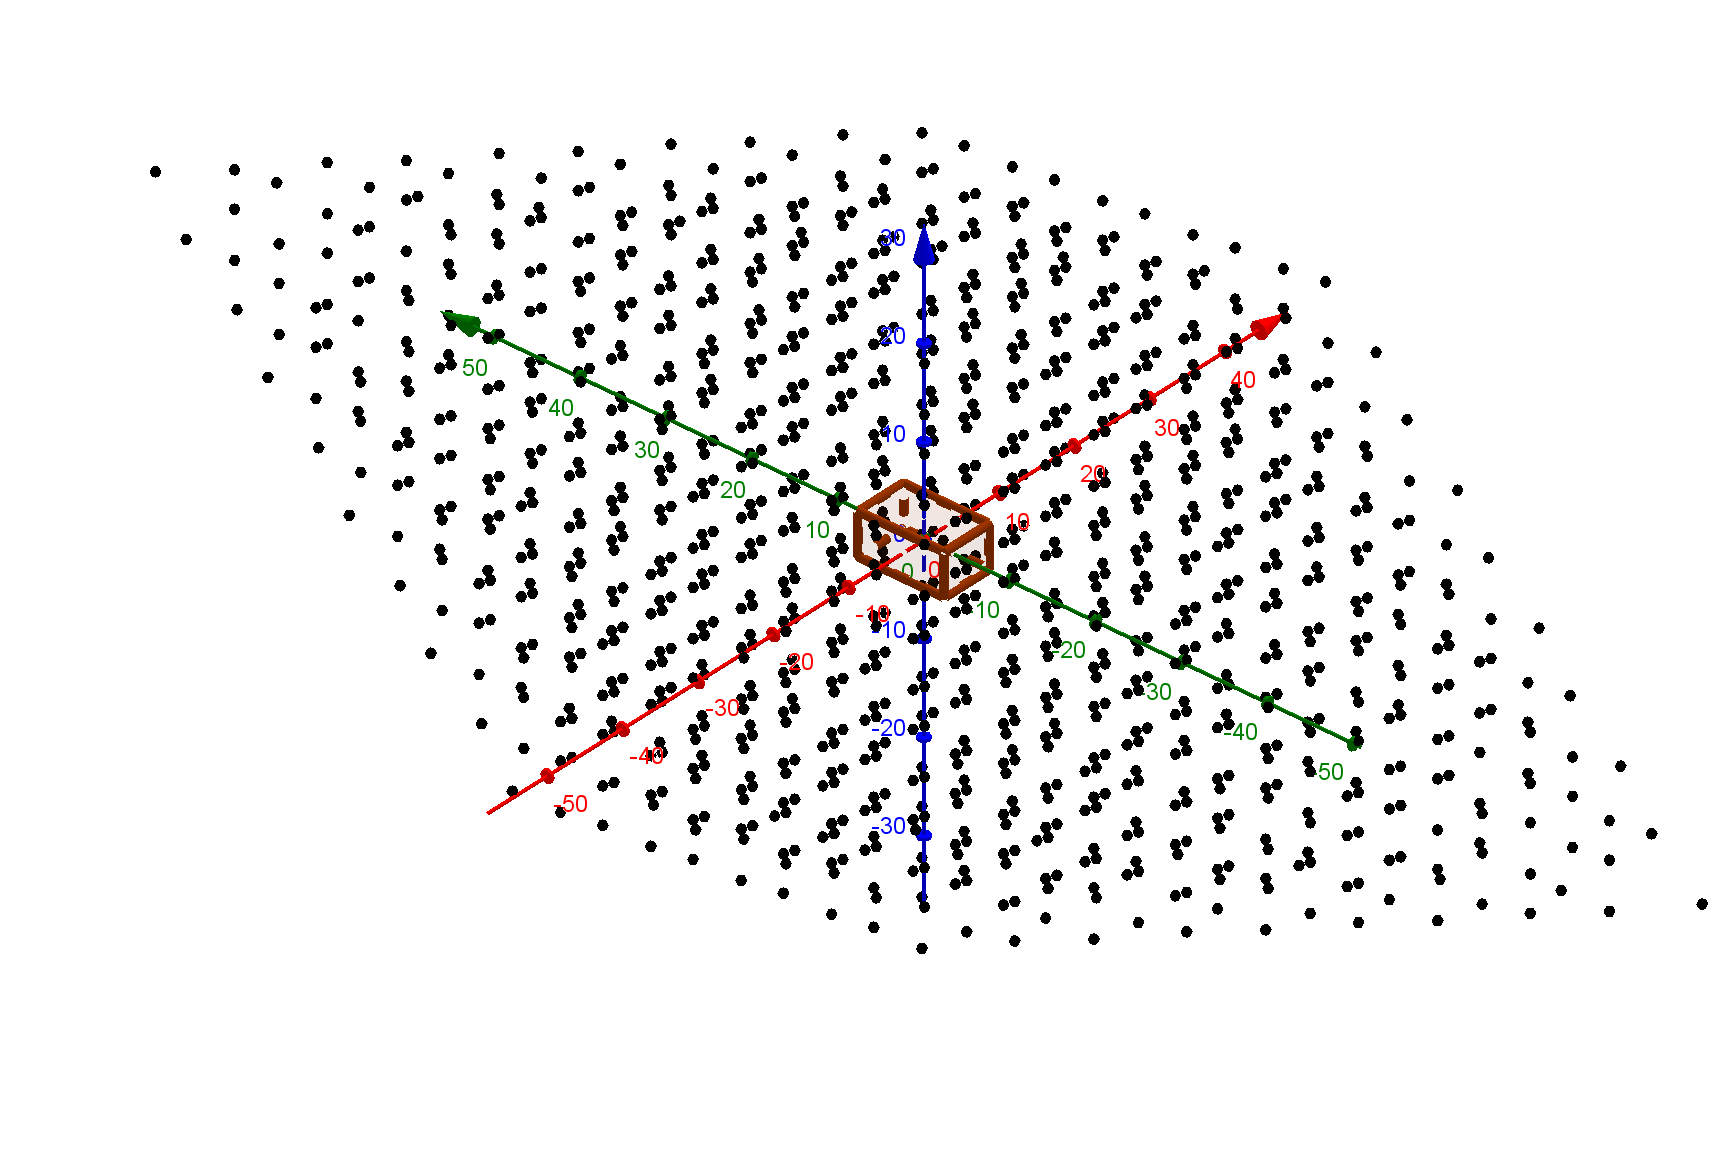
\includegraphics[width=12cm]{rys11}
	\caption{Siatka źródeł pozornych.}
\end{figure}













